\section{Algorithms and Implementation Details}
\label{sec:imp}
In this section, we summarize the entire algorithm and explain the implemented details.\\ 
\subsection{Algorithm}
Based on our formulation in section \ref{sec:method}, our algorithm can be summarized as in Algorithm \ref{alg:jrcs}.
\begin{algorithm}[htb]
	\caption{Joint Registration and Co-segmentation (JRCS)}
	\label{alg:jrcs}
	\textbf{Input:}~~\\
	$\{V_m\}$:$M$ input 3D point sets\\
	$\Theta^0$:Initial parameters~~\\
	$\{\beta_{ik}\}_{m}$:layout based prior\\
	\textbf{Output:}~~\\
	$\Theta^q$:Final parameters~~
	\begin{enumerate}
		\item $q\leftarrow1$
		\item \textbf{repeat}
		\item E-step: Use $\Theta^{q-1}$ to estimate $\alpha_{mik}^q$ according to (\ref{equ:estep}) ( (\ref{equ:bestep}) if use bilateral formulation)
		\item alter $\alpha_{mik}^q$ with $\{\beta_{ik}\}_{m}$ according to (\ref{equ:alteralpha})
		\item M-step-a: Use $\alpha^q_{mik}$, $\pmb x^{q-1}_k$ to estimate $\{R_{mn}^q\}$ and $\{\pmb t_{mn}^q\}$ according to (\ref{equ:updateR})(\ref{equ:updatet})
		\item M-step-b: Use $\alpha^q_{mik}$, $\{R_{mn}^q\}$ and $\{t_{mn}^q\}$ to update other parameters for Gaussian models according to (\ref{equ:updatexk})(\ref{equ:updatesigma})(\ref{equ:updatepk})(\ref{equ:updatey})  ( and (\ref{equ:updatefk})(\ref{equ:updatefsigma}) if use bilateral formulation)
		\item $q \leftarrow q+1$
		\item \textbf{until} Convergence
		\item \textbf{return} $\Theta^q$
	\end{enumerate}
\end{algorithm}
\subsection{Implementation Details}
\textbf{Initialization of $\Theta$}:\\
We first determine the total number of Gaussian model $K_{all}$ as we explained in subsection \ref{sec:imp:interact}. We set $p_k=\frac{1}{\sum K_n}$ which means each Gaussian model have the same weight at the beginning. We seperate the Gaussian models into $N$ groups to represent $N$ objects. Each group has $K_n$ Gaussian models based on (\ref{equ:K_n}). $\{\pmb x_k\}_n$ are Gaussian centroids of $n^{th}$ group and they are initialized as a random positions uniformally distributed on the surface of a sphere. The radius of the sphere is chosen as the median of the radius of the input point sets $r$. The center of the $n^{th}$ spheres is $c_n=(0,0,z_n)$, where $z_n\in \{-(N-1)r,-(N-3)r,...,(N-1)r\}$. This means that the object models are vertically arranged in latent space as shown in Figure~\ref{fig:teaser}(c) and in Figure~\ref{fig:localoptimal}(b).We choose vertical arrangement for groups of object merely for the convenience of visualization. We choose the sphere as the initial shape so that we can initialize all the $R_{mn}$ to identity matrix. For the $\pmb t_{mn}$ we initialize them as $\pmb t_{mn}=- \pmb c_n$ so that all the object model starting with position at origin point when they are transformed to the space of each input set. However, if the $m^{th}$ input point set has the manually placed layout, we treat the associated $\pmb t_{mn}$ differently. For this case we have:
\begin{equation}
\label{equ:initt}
\pmb t_{mn}=\frac{\sum_{\pmb v_{mi} \in B_n}\pmb v_{mi}}{N(B_n)}-\pmb c_n
\end{equation}
where $N(B_n)$ is the number of element in $B_n$ and $B_n$ is the point set that is enclosed by the mannual input layout (boxes). 
\subsection{Hot Intervention Machinism}
Our current implementation of optimization is quite slow (fail to converge in interative time) especially when the point numbers inside each input point set are large and it is possible for our optimization to stuck in a local optimal, requiring the guide from the mannual input. As a compensation for these drawbacks. We implement a hot intervention machinism, allowing the mannaul input take effect even after the optimization has started. Theoretically, this is possible due to the i.i.d assumption. 
This assumption makes it possible for the calculation of posterior probability being independent for each input point set. Even after the optimization is started, we can still allow the user to add more layouts for other point sets and the program can do the same alteration as (\ref{equ:alteralpha}) in the next iteration. The Figure~\ref{fig:hi} shows how the users can use the hot intervention machinism within our tool.
\begin{figure}[htb]
	\centering
	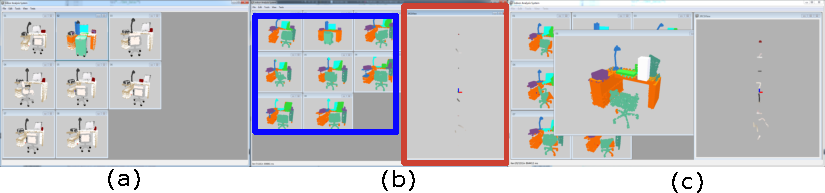
\includegraphics[width=\linewidth]{images/hotintervention/hi}
	\caption{\label{fig:hi}This figure shows the hot intervention machinism. (a) is the input point sets with mannually placed layout in 2rd point set. (b) shows that from the region highlighted by blue rectangle the user can see the instant result of segmentation and from the region highlighted by the red rectangle the user can see the space of object model(the shape of the centroids of the Gaussian models). (c) shows that the user picks another input point set and adds more boxes targeting the incorrect segmentation to further guide the optimization when the optimization is running.}
\end{figure}
 